\chapter{Implementierung}
% TODO: Dieses Kaptiel mit der Zeit anpassen

\section{Existierende Frameworks}

\subsection*{WRLD SDK}

Das \emph{WRLD SDK}\footnote{\url{https://www.wrld3d.com/}} (fortan \enquote{WRLD}) ein Framework, um interaktive 3D-Karten zu erstellen und anzuzeigen.
Es unterstützt mehrere Plattformen und bietet zudem ein Plugin für Unity an.
WRLD bezieht dabei seine Kartendaten von \emph{OpenSteetMap} sowie diversen proprietären Anbietern \parencite{WRLD2018}.
Die Daten werden aufbereitet und Nutzern über WRLDs eigene Server zur Verfügung gestellt.
Eine AR-Beispielanwendung ist in \autoref{fig:wrld_ar} zu sehen.
\begin{figure}[h]
    \centering
    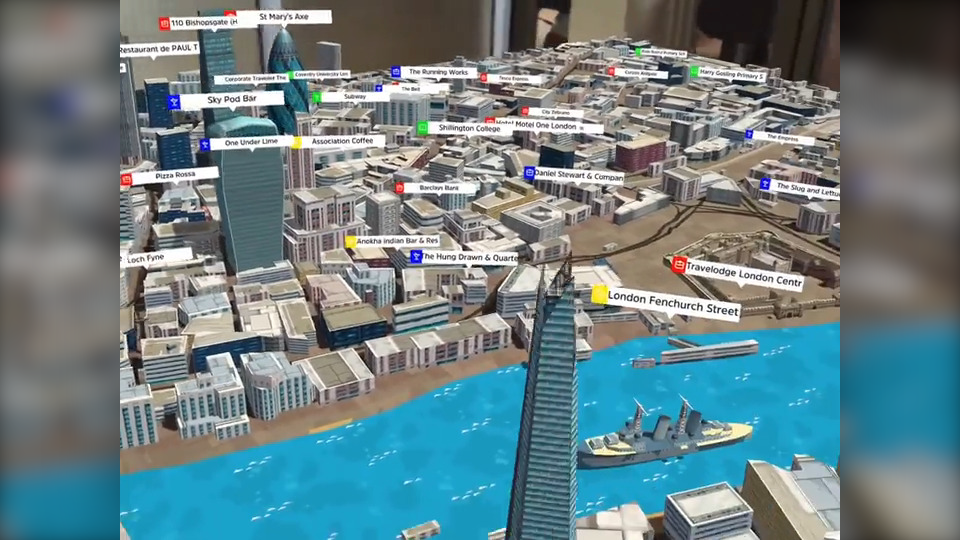
\includegraphics[width=\linewidth]{figures/wrld_ar-web-11_wide}
    \caption{AR-Anwendung von WRLD, welche eine 3D-Ansicht von London auf einem Tisch platziert. \quelle{\cite{WRLD2018b}}}
    \label{fig:wrld_ar}
\end{figure}

Das Besondere an WRLD ist, dass es eine Funktion zur Einbettung von Indoor-Karten von Gebäuden bietet.
Hierzu können Entwickler georeferenzierte Lagepläne auf die WRLD-Server hochladen und für das gewünschte Gebäude registrieren.
Danach sind die Indoor-Karten für die Gebäude öffentlich für alle Nutzer von WRLD zugänglich.
Zudem können die Indoor-Karten mit Einrichtungsgegenständen versehen werden, um die Karten natürlicher aussehen zu lassen.
\autoref{fig:wrld_indoor} zeigt die Interaktion mit WRLDs Indoor-Karten.
In der Karten-3D-Ansicht kann über einen Button das Gebäude betreten werden (falls eine Indoor-Karte für das Gebäude vorhanden ist).
Über einen Slider kann das anzuzeigende Stockwerk ausgewählt werden.
Dabei werden alle Stockwerke des Gebäudes mit einer Animation aufgefächert und mit dem Slider durchlaufen.
Schließlich wird das ausgewählte Stockwerk angezeigt.
Alle Stockwerke oberhalb des Aktuellen werden ausgeblendet, die darunterliegenden werden durch das Aktuelle überdeckt.
\begin{figure}[h]
    \begin{subfigure}{0.49\textwidth}
        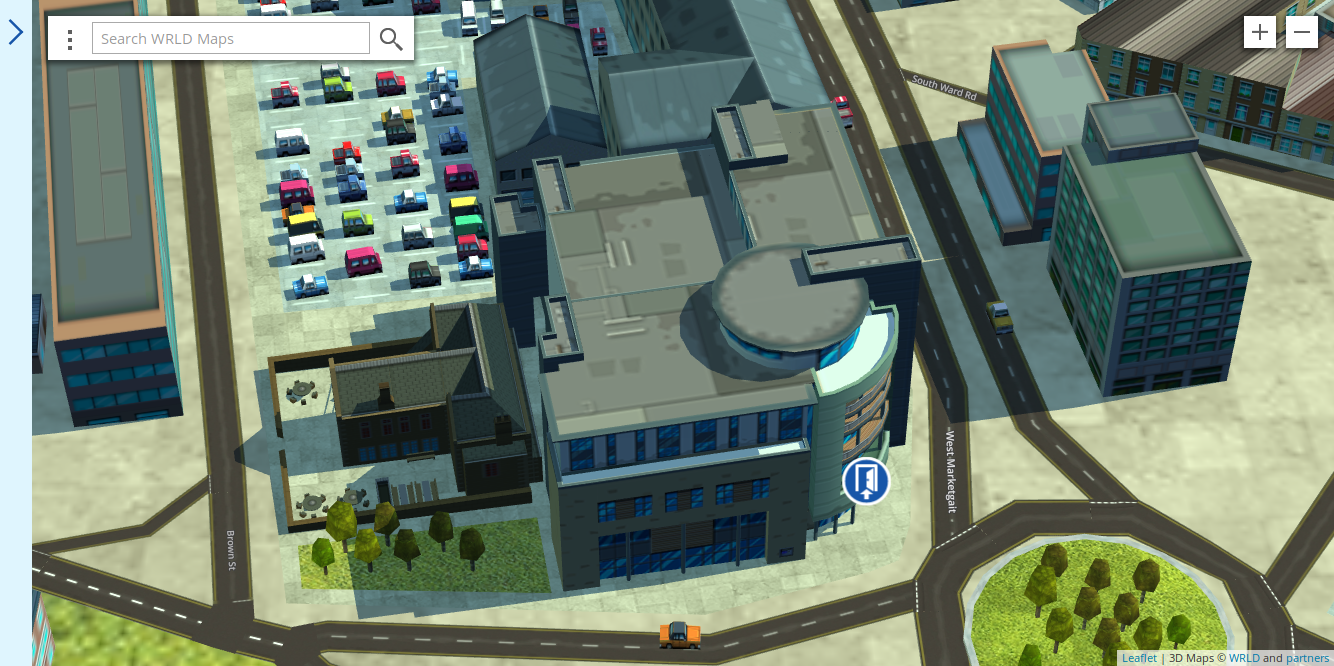
\includegraphics[width=\textwidth]{figures/wrdl_outdoor.png}
        \caption{}
        \label{sfig:wrld_outdoor}
    \end{subfigure}
    \hfill
    \begin{subfigure}{0.49\textwidth}
        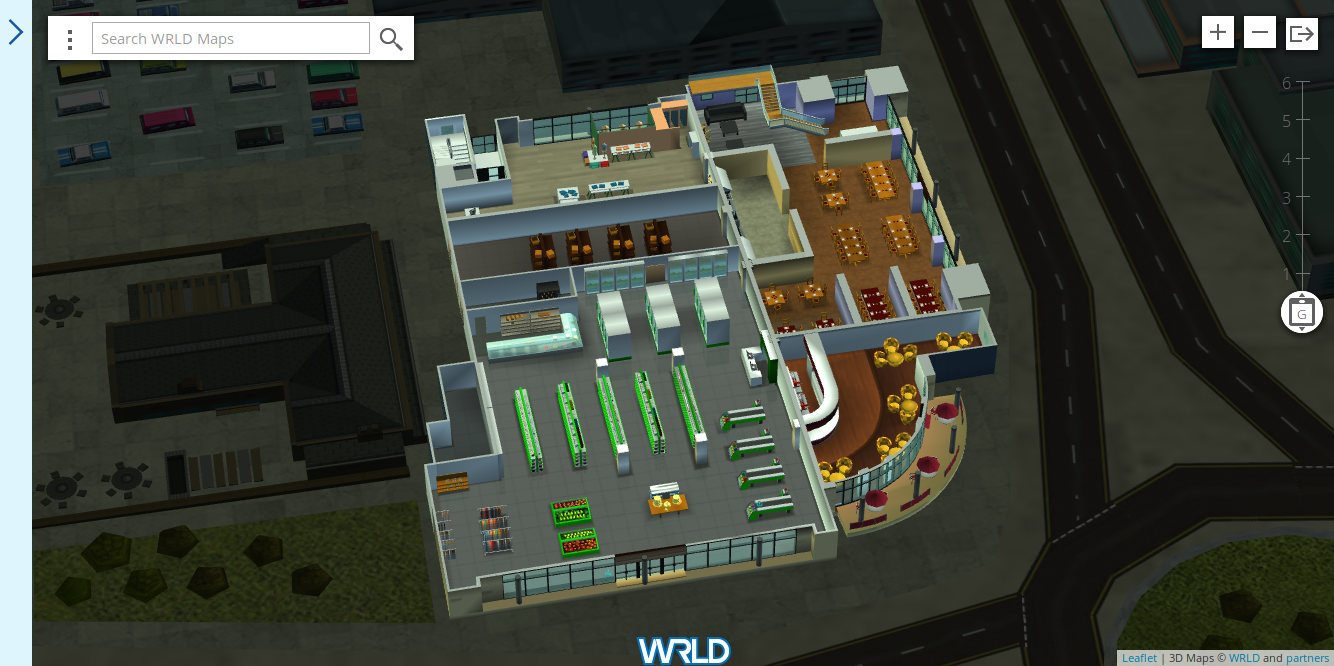
\includegraphics[width=\textwidth]{figures/wrdl_indoor_g.png}
        \caption{}
        \label{sfig:wrld_indoor_g}
    \end{subfigure}
    \newline
    \begin{subfigure}{0.49\textwidth}
        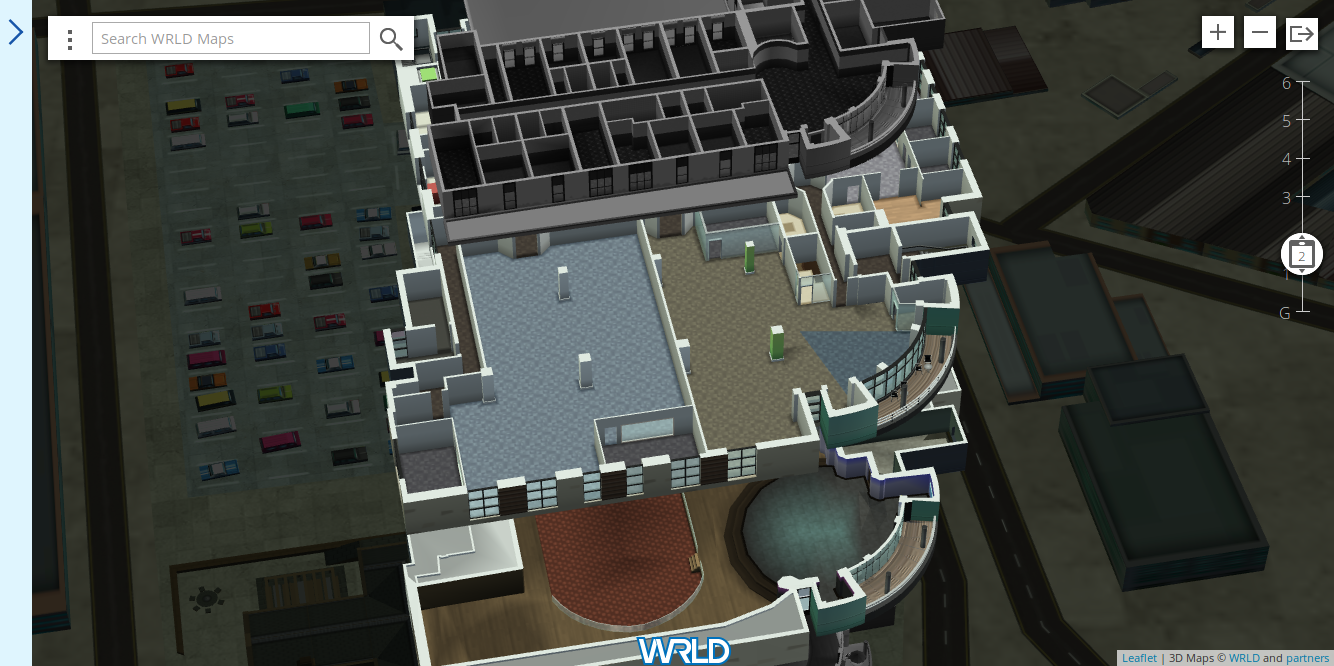
\includegraphics[width=\textwidth]{figures/wrdl_indoor_transition.png}
        \caption{}
        \label{sfig:wrld_indoor_transition}
    \end{subfigure}
    \hfill
    \begin{subfigure}{0.49\textwidth}
        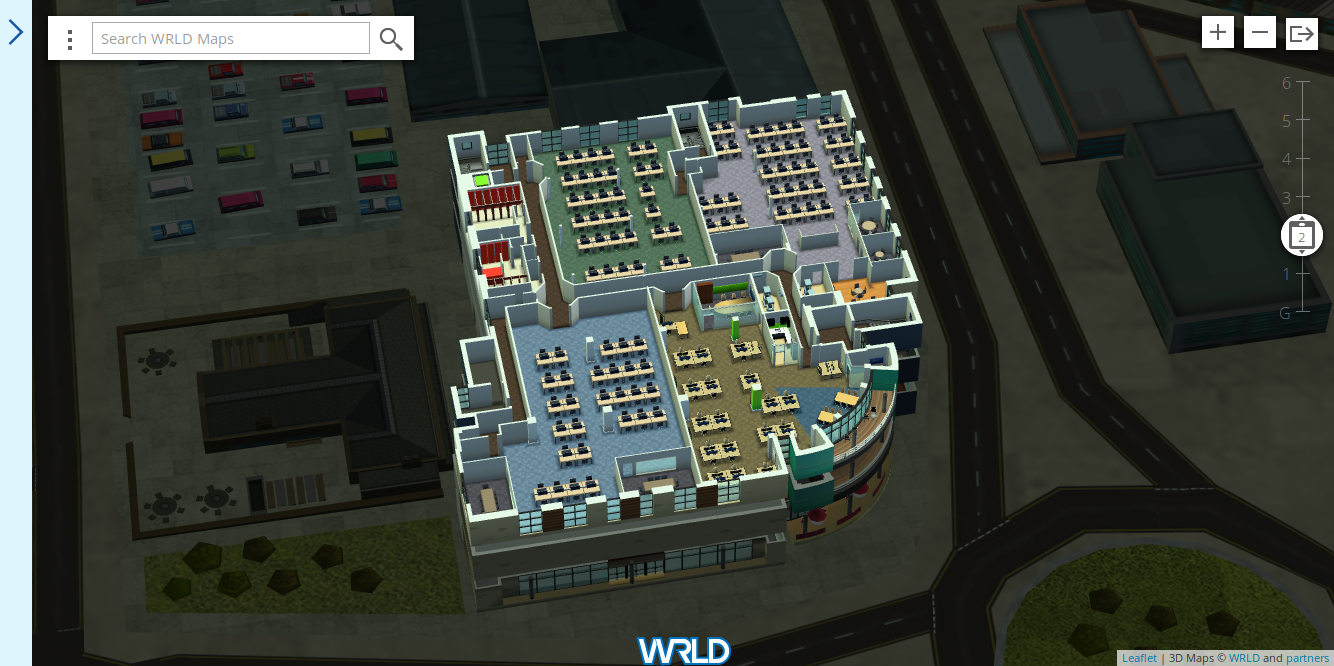
\includegraphics[width=\textwidth]{figures/wrdl_indoor_2.png}
        \caption{}
        \label{sfig:wrld_indoor_2}
    \end{subfigure}
    \caption{Indoor-Funktionalität von WRLD. %
        \subref{sfig:wrld_outdoor} Das Gebäude ist von außen sichtbar. %
        Über einen Button kann das Gebäude betreten werden. %
        \subref{sfig:wrld_indoor_g} Die Innenansicht des Gebäudes mitsamt Einrichtung wird angezeigt. %
        \subref{sfig:wrld_indoor_transition} Über einen Slider können die Stockwerke gewechselt werden. %
        \subref{sfig:wrld_indoor_2} Untenliegende Stockwerke werden vom aktuellen Stockwerk verdeckt.%
    }
    \label{fig:wrld_indoor}
\end{figure}

Für das Ziel dieser Arbeit (die Implementierung einer Indoor-Megamap im Stil von TCTD) wäre WRLD durch seine Indoor-Funktionalität eine ideale Grundlage.
Allerdings hat das SDK einen Nachteil, welches den Einsatz für diese Arbeit unmöglich macht.
Um eine Indoor-Karte in das SDK einzubinden, muss diese für das entsprechende Gebäude auf die WRDL-Server hochgeladen werden.
Im Fall dieser Arbeit wäre das eine Indoor-Karte für das MZH der Universität Bremen.
WRLDs Kartenabdeckung für Deutschland ist jedoch nur teilweise vorhanden; die Daten für Bremen fehlen komplett.
Das MZH steht somit beim Upload der Karte nicht zur Verfügung.
Die Recherche des Verfassers dieser Arbeit ergab keine Möglichkeit, den Upload auf die Server durch eine Offline-Nutzung des SDKs zu umgehen.
Daher muss bei der Implementierung der Megamap auf WRLD verzichtet werden.
Die Art der Darstellung und Integration der Indoor-Karte in die Umgebung sowie der Wechsel zwischen den Stockwerken dient jedoch als Inspiration für die Implementierung einer eigenen Lösung.

\subsection*{Mapbox SDK}
% TODO: Grafik für nicht funktionierende Pipeline?

%
\cleardoublepage